\documentclass[
tikz,
border=5pt,
convert={density=600,
	outext=.png
}
]{standalone}


\usepackage[utf8]{inputenc}
\usepackage{stanli}
\usepackage{tikz}
\usetikzlibrary{arrows.meta,arrows,positioning,calc,backgrounds}

\begin{document}

\setcoords{-25}{30}[1][1] 
\setaxis{2} 
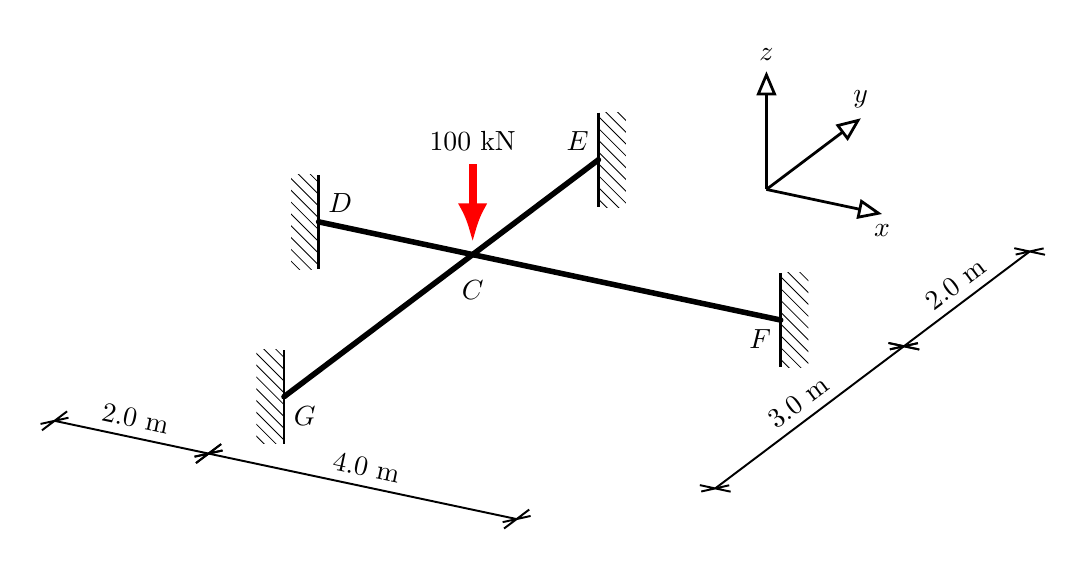
\begin{tikzpicture}[coords, background rectangle/.style={fill=white!45}, show background rectangle]

    \dpoint{c}{0}{0}{0};
    \dpoint{d}{-2}{0}{0}; 
    \dpoint{e}{0}{2}{0}; 
    \dpoint{f}{4}{0}{0};
    \dpoint{g}{0}{-3}{0}; 
    \dpoint{z}{ 0.7*3.0 }{ 1.05*2.0 }{0}; 

    \daxis{1}{z}; 

    \foreach \startn/\endn in {c/d,c/e,c/f,c/g}
        \dbeam{1}{\startn}{\endn};

    \support{3}{d}[270];
    \support{3}{e}[90];
    \support{3}{f}[90];
    \support{3}{g}[270];

    \begin{scope}[force/.append style={color=red,>={Latex[length=0pt 5]}},
    normalLine/.append style={line width=1mm}]
        \dload{1}{c}[0][90];
        \dnotation{1}{c}{$100$~kN}[above=12mm];
    \end{scope}

    \ddimensioning{yx}{g}{c}{1.4*4.0}[$3.0$~m];
    \ddimensioning{yx}{c}{e}{1.4*4.0}[$2.0$~m];
    \ddimensioning{xy}{d}{c}{-1.4*3.0}[$2.0$~m];
    \ddimensioning{xy}{c}{f}{-1.4*3.0}[$4.0$~m];

    \dnotation{1}{c}{$C$}[below=2mm];
    \dnotation{1}{d}{$D$}[above right];
    \dnotation{1}{e}{$E$}[above left];
    \dnotation{1}{f}{$F$}[below left];
    \dnotation{1}{g}{$G$}[below right];

\end{tikzpicture}
        
\end{document}
